%Dokumententyp
\documentclass[a4paper]{article}

\usepackage[a4paper,left=2cm, right=3cm, top=2cm]{geometry}

%Kodierung
\usepackage[utf8]{inputenc}
\usepackage[T1]{fontenc}

%Grafiken einbinden
\usepackage{graphicx}
\usepackage{subfigure} 

%Position von Grafiken und Tabellen erzwingen:
\usepackage{float}

%URLs im Literaturverzeichnis
\usepackage{url}

\usepackage{amsmath}

%Vektoren einfacher angeben:
\newcommand{\vektor}[1]{\left( \begin{array}{c} #1 \end{array} \right) }


%Schriftart Arial:
% \usepackage{helvet}

%Figures with text around it:
\usepackage{wrapfig}

\usepackage{listings}

%seitennummern rechts:
% \usepackage{fancyhdr}
% \fancyhf{} % clear all header and footers
% \renewcommand{\headrulewidth}{0pt} % remove the header rule
% \rfoot{\thepage}
% \fancypagestyle{plain}{%redefining plain pagestyle
% \fancyhf %clear all headers and footers fields
% \fancyhead[R]{\thepage} %prints the page number on the right side of the header
% }

%Schriftart Times New Roman "like"
\usepackage{txfonts}

%Sprache
\usepackage[german]{babel}

%Checkmarks: (usage: \checkmark)
\usepackage{dingbat}

\usepackage{listings}
\usepackage{color}
\definecolor{javared}{rgb}{0.6,0,0} % for strings
\definecolor{javagreen}{rgb}{0.25,0.5,0.35} % comments
\definecolor{javapurple}{rgb}{0.5,0,0.35} % keywords
\definecolor{javadocblue}{rgb}{0.25,0.35,0.75} % javadoc
 
\lstset{language=Java,
basicstyle=\ttfamily,
keywordstyle=\color{javapurple}\bfseries,
stringstyle=\color{javared},
commentstyle=\color{javagreen},
morecomment=[s][\color{javadocblue}]{/**}{*/},
numbers=left,
numberstyle=\tiny\color{black},
stepnumber=1,
numbersep=5pt,
tabsize=4,
showspaces=false,
lineskip={-1.5pt},
showstringspaces=false}

%Tabellenextras
\usepackage{tabularx}

%Zeilenabstand 1.5
\linespread{1.5}
\usepackage{setspace}

%Figure Captions mit Fußnoten
\usepackage{footnote}
%\setlength{\parindent}{0pt} 

%Graphen/Trees zeichnen:
\usepackage{tikz}
\newcommand*\circled[1]{\tikz[baseline=(char.base)]{
            \node[shape=circle,draw,inner sep=2pt] (char) {#1};}}


%itemize items richtig ausrichten (nicht links überlappen!)
% \setlist{leftmargin=0}

% %%%%TITELSEITE%%%%%%(
% \title{ Konzept und Implementierung\\ eines Systems zur \\Anforderung und Verwaltung von virtuellen privaten Clustern}
% \author{\textbf{\large Bachelorarbeit}}
% 
% \date{zur Erlangung des akademischen Grades Bachelor of Science an der Universität Paderborn im Fachbereich Informatik im Studiengang Bachelor Informatik}

% %%%%TITELSEITE%%%%%%)

% \pagestyle{fancy}
\begin{document}

\title{Algorithmische Geometrie - Sommersemester 2015\\
       8. Aufgabenblatt }
\author{Simon Koennecke und Felix Bröker}
\date{}
\maketitle

\section*{Aufgabe 1 - Vorverarbeitungszeit für Bereichsbäume}

Im folgenden sehen wir uns zunächst in Pseudocode an, 
wie ein 2d-Bereichsbaum aufgebaut werden kann:

\begin{lstlisting}
Eingabe: pX, pY (nach x- bzw. y-Koordinate sortiertes Array der Punkte aus P)
Ausgabe: Wurzelknoten des 2d-Bereichbaums

Create-2d-Range-Tree(pX, pY)
IF size(pX) == 0
	return NULL;
ELSE
	yTree = Create-1d-Range-Tree(pX, pY);

IF size(pX) == 1
	return new Node(pX[1], yTree, NULL, NULL);
ELSE
	pY1 = updatepY(pX[1..ceiling(size(pX)/2)], pY);
	pY2 = updatepY(ceiling(pX[size(pX)/2)+1..size(pX)], pY);
	leftNode  = Create-2d-Range-Tree(pX[1..ceiling(size(pX)/2)], pY1);
	rightNode = Create-2d-Range-Tree(ceiling(pX[size(pX)/2)+1..size(pX)], pY2);
	return new Node(ceiling(pX[size(pX)/2]), yTree, leftNode, rightNode);
\end{lstlisting}

Die 4 Parameter von "`Node"' geben dabei den zu speichernden x-Wert (der jeweilige Median), 
den zum Knoten zugehörigen 1d-Bereichsbaum (bzgl. der y-Koordinaten der zugehörigen Punkte),
den linken, sowie rechten Kindknoten an. "`Create-1d-Range-Tree(pX, pY)"' erstellt einen 1d-Bereichsbaum für alle Punkte in pX nach deren y-Koordinate. 
Die Funktion updatepY(pX, pY) reduziert die Menge pY jeweils um die nicht in pX enthaltenen Punkte.
Dieser Vorgang benötigt $\mathcal{O}(size(pX))$ viele Operationen.

\subsection*{Laufzeitabschätzung}
Zur Laufzeitabschätzung stellen wir folgende Rekursionsgleichungen auf:
$$T(\leq 1) = \mathcal{O}(1)$$
Im Fall von $n \leq 1$ (Rekursionsanker) haben wir eine konstante Laufzeit.
Dies können wir auch an obigem Pseudocode ablesen. Ist die Eingabegröße $ n < 1$ bzw. $n = 0$
wird lediglich ein "`NULL"'-Element zurückgegeben. Im Fall $n = 1$ wird lediglich ein neuer Knoten
und dessen 1-elementiger 1d-Range-Tree (ebenfalls konstante Zeit) angelegt und zurückgegeben. 
In allen anderen Fällen setzt sich die Laufzeit aus der Zeit für die Konstruktion eines 1d-Range-Trees
(Zeile 8), der Zeit zur Reduzierung der Menge pY (Zeilen 13, 14), der Zeit für den Aufruf beider Rekursionen (Zeilen 15,16) und der Erstellung des Rückgabeknotens (Zeile 17) zusammen:

$$T(n) = T(\lfloor n/2\rfloor) + T(\lceil n/2\rceil) + \underbrace{\mathcal{O}(n) + \mathcal{O}(n) + \mathcal{O}(1)}_{\mathcal{O}(n)}$$

Der 1d-Range-Tree kann mithilfe der 
sortierten Liste pY in O(n) Zeit konstruiert werden. Die grobe Idee zur Lösung in O(n) lässt sich 
wie folgt beschreiben: Es werden je zwei der Knoten am Anfang der Liste entnommen, der entsprechende
Elternknoten erstellt und dieser am Ende der Liste wieder eingefügt, solange bis nur noch ein Knoten
in der Liste enthalten ist. Da die Menge der Knoten eines binären Baums in $\mathcal{O}(n)$ liegt, 
benötigt diese Prozedur ebenfalls $\mathcal{O}(n)$ Zeit. 

 Die Zeit für die Erstellung des Rückgabeknotens inklusive anderer
konstanter Operationen wie z.B. der verwendeten IF-Abfragen kann mit $\mathcal{O}(1)$ abgeschätzt
werden. Da die aktuelle Punktemenge der Größe $n$ anhand ihres Medians geteilt und als Eingabe der
nächsten Rekursionen verwendet werden, und nicht sicher ist, ob $n$ eine 2er-Potenz ist, werden
jeweils die auf- bzw. abgerundeten Hälften der Eingabegröße zur Abschätzung ($T(\lfloor n/2\rfloor)$  und $T(\lceil n/2\rceil)$) verwendet. 

Die aufgestellte Rekursionsgleichung entspricht genau der Rekursionsgleichung wie wir sie von Sortieralgorithmen wie z.B. Mergesort kennen. Für Mergesort ist die Laufzeitabschätzung 
$T(n) = \mathcal{O}(n \log n)$ bekannt. Die hier vorgestellte Berechnung/Konstruktion eines
2d-Range-Trees benötigt also ebenfalls $\mathcal{O}(n \log n)$ Zeit.

\section*{Aufgabe 2 - dynamische Segmentbäume}
Wir haben ein Universum $U$ mit $|U| = N$ gegeben. Sei weiterhin ein dynamischer Segmentbaum in Form eines AVL-Baums über diesem Universum gegeben. Dieser beinhaltet bereits eine Menge $I$ von Intervallen. 

Im Folgenden beschreiben wir zunächst das \textbf{Einfügen} eines neuen Intervalls $I_n = [a,b]$:

\begin{itemize}
 \item Fall 1 ( $a \in U \wedge b \in U$ ): 
    Füge $I_n$ nach bekannter Prozedur in den Segmentbaum ein. Dies geht bekanntermaßen 
    in $\mathcal{O}(\log N)$ Zeit.
 \item Fall 2 ( $a  \notin U \vee b  \notin U$)
    \begin{itemize}
     \item Erweitere das Universum $U$ wie folgt: $U = U \cup \left\{a,b\right\}$
     \item Für jedes neue Element $x \in \{a,b\}$ führe jeweils folgende Schritte aus:
     
	\begin{figure}[!htb]
	   		\subfigure[Elternknoten ein $\leq$ Knoten ($b$ durch gestrichelte Linie gekennzeichnet)]{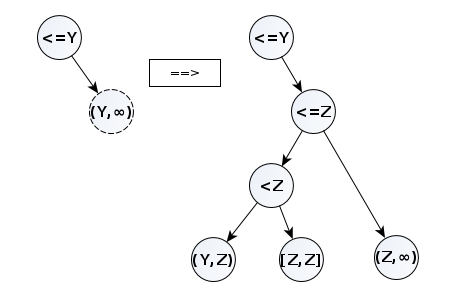
\includegraphics[width=0.5\textwidth]{aufgabe02_1}} 
   		\subfigure[Elternknoten ein $<$ Knoten ($b$ durch gestrichelte Linie gekennzeichnet)]{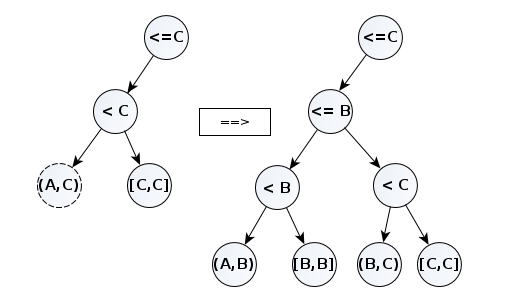
\includegraphics[width=0.5\textwidth]{aufgabe02}} 
	\end{figure} 
	
     \begin{enumerate}
     	\item Führe eine Binärsuche nach $x$ durch. Wir landen dabei in einem Blattknoten $b$
     	mit einem offenen Intervall $(i,j)$. 
     	\item Wir entfernen $b$ aus dem Baum, merken uns jedoch den Elternknoten $p(b)$ 
     	und die Knotenliste $b_{KL}$ von $b$.
     	\item Wir erstellen neue Knoten für die Intervalle $(i,x)$, $[x,x]$ und $(x,j)$
     	\item Weiterhin erstellen wir die Knoten "`$\leq x$"' und "`$< x$"'.
     	\item Falls $p(b)$ ein "`$<$"'-Knoten ist, entfernen wir die Knotenliste $p(b)_{KL}$ von $p(b)$
     	und fügen sie zum Knoten "`$\leq x$"' hinzu.
     	\item Alle neu erstellten Knoten bis auf "`$(x,j)$"' speichern wir nun in einer Liste $L$ mit folgender Reihenfolge:
     	L = \circled{$\leq x$}, \circled{$< x$}, \circled{$(i,x)$}, \circled{$[x,x]$}
     	\item Falls $p(b)$ ein "`$<$"'-Knoten ist, entnehmen 
     	wir den Knoten $p(b)$ und seinen rechten Kindknoten $rc(p(b))$ aus dem Baum und fügen sie
     	in dieser Reihenfolge am Ende der Liste $L$ ein. 
     	\item Nun fügen wir auch "`$[x,j]$"' am Ende der Liste $L$ ein.
     	\item Schließlich durchlaufen wir die Liste $L$ vom Anfang bis zum Ende und fügen 
     	die entsprechenden Knoten nacheinander in den AVL-Baum ein. 
     	
     	Die Abbildungen (a) und (b) illustrieren die Änderungen, welche im Fall eines "`$\leq$"'- 
     	und eines "`$<$"'-Elternknotens $p(b)$ bewirkt werden.
     	
     	\item Um eine richtige Verteilung der ursprünglichen Intervalle im aktualisierten
     	Segmentbaum sicherzustellen, wenden wir noch folgende Operation an: 
     	Wir interpretieren den Knoten "`$\leq x$"' als Wurzelknoten eines eigenen Segmentbaums und
     	fügen nacheinander alle Intervalle $I_b$ der Knotenliste $b_{KL}$, welche wir uns zuvor gemerkt haben, in dem "`Segmentbaum"' "`$\leq x$"' ein.
     	\item Insgesamt ist der aktualisierte Baum nun wieder in einem gültigen Zustand bzgl. des 
     	aktualisierten Universums $U$ und der zuvor bereits gespeicherten Intervalle $I$.
     	\item Das neue Intervall $I_n = [a,b]$ kann nun nach der bekannten Prozedur 
     	in $\mathcal{O}(\log N_n)$ ($N_n$ ist Größe des aktualisierten Universums $U$) Zeit im Baum eingefügt werden.

     \end{enumerate}
\end{itemize}

Zum \textbf{Streichen} eines Intervalls $I_a = [a,b]$ aus dem Segmentbaum gehen wir wie folgt vor:

\begin{itemize}
	\item Fall 1 ($\exists I_i = [a_i, \_] \in U, \exists I_j = [\_, b_j] \in U: \qquad a = a_i \wedge b = b_j \wedge I_i \neq I_a \wedge I_j \neq I_a $):
	
	Streiche $I_a$ nach bekannter Prozedur aus dem Segmentbaum. Dies geht bekanntermaßen in 
	$\mathcal{O}(\log N)$ Zeit. 
	\item Fall 2 ($\neg(\exists I_i = [a_i, \_] \in U, \exists I_j = [\_, b_j] \in U: \qquad a = a_i \wedge b = b_j \wedge I_i \neq I_a \wedge I_j \neq I_a )$):
	
	In diesem Fall streichen wir zunächst ebenfalls $I_a$ nach bekannter Prozedur aus dem Segmentbaum.
	Allerdings existieren nun ein oder zwei Punkte $x \in \{a,b\}$, welche nicht mehr Intervallendpunkt
	irgendeines verbliebenen Intervalls $I_i$ sind. D.h., der aktuelle Segmentbaum speichert diese
	Punkte $x$ unnötigerweise, was einen höheren Speicherbedarf der Datenstruktur bedeutet.
	Deshalb beschreiben wir im Folgenden, wie wir nun jeweils auch einen solchen Punkt $x$ aus dem Segmentbaum
	entfernen:
	
	\begin{enumerate}
		\item Zunächst aktualisieren wir $U$ mit $U = U\setminus \{x\}$
		\item 
	\end{enumerate}
\end{itemize}

\end{itemize}






\section*{Aufgabe 3 - Punkt-Rechteck-Anfragen}

\subsection*{Datenstruktur}
Als Datenstruktur für effiziente Punkt-Rechteck-Anfragen verwenden wir einen Segmentbaum, 
welcher in seinen Knoten nicht auf Listen, sondern auf weitere Segmentbäume verweist.
Der primäre Segmentbaum ist über den x-Intervallen der $n$ Rechtecke definiert. 
Dabei ist das Universum $U$ des Segmentbaums als die Vereinigung aller Intervall-Endpunkte
der x-Intervalle gegeben. 

Die in einem "`gewöhnlichen"' Segmentbaum vorhandenen Listen geben Aufschluss über die 
Intervalle, in denen ein Punkt der Anfrage liegt. Wir ersetzen diese Listen von 
x-Intervallen jeweils durch einen Segmentbaum, welcher alle y-Intervalle enthält, 
die zu denselben Rechtecken gehören wie die x-Intervalle der ursprünglichen Liste.

Auf diese Weise kann bei einer Anfrage direkt an einem Knoten effizient ermittelt werden, 
in welchen Rechtecken sich der Punkt befindet. 


\subsubsection*{Vorverarbeitungszeit}
Um die beschriebene Datenstruktur zu erhalten, konstruieren wir zunächst einen
"`gewöhnlichen"' Segmentbaum $S$ über dem Universum $U$ und allen 
$n$ x-Intervallen. Da die Größe von $U$ in unserem Fall 
lediglich Endpunkte der $n$ x-Intervalle umfasst und somit in $\mathcal{O}(n)$ liegt, 
kann die Laufzeit zur Konstruktion mit $\mathcal{O}(n \log n)$ abgeschätzt werden.

Anschließend traversieren wir den Baum $S$ und ersetzen an jedem Knoten $k$ (falls vorhanden)
die Liste der zugehörigen x-Intervalle $k_L$ durch einen Verweis auf 
den Segmentbaum $sY$, welcher die korrespondierenden y-Intervalle der (zu den x-Intervallen 
gehörenden) Rechtecke beinhaltet. Das Traversieren benötigt dabei $\mathcal{O}(n)$ Zeit.
Die Konstruktion eines Segmentbaums $sY$ benötigt ....
TODO: Hier berechnen, wie lange es dauert, für alle maximal n * 2 log n Intervalleinträge
Segmentbäume aufzubauen...

TODO: Insgesamtlaufzeit ,also O(n log n) + O(n) + O(??) = O(???)... angeben.. 

\subsubsection*{Speicherbedarf}
Der Speicherbedarf für den "`gewöhnlichen"' Segmentbaum liegt  in $\mathbb{O}(n \log n)$ (Beachte: Das Universum $U$ ist nur über den Endpunkten der x-Intervalle
definiert/konstruiert). Hinzu kommt der Speicherbedarf für alle Segmentbäume $sY$.
Dieser lässt sich wie folgt abschätzen:

\begin{itemize}
	\item In der Vorlesung wurde gezeigt, dass jedes Intervall im Segmentbaum maximal $2 * h$- mal (h ist die Höhe des Segmentbaums), also in unserem Fall $2 * h = 2 * \log n 
	= \mathcal{O}(\log n)$ häufig in einer Knotenliste auftreten kann.
	\item Da wir $n$ x-Intervalle haben, haben wir im gesamten Baum maximal $\mathcal{O}(n \log n)$ viele
	Eintragungen von Intervallen in Knotenlisten.
	\item Da nun die korrespondierenden $\mathcal{O}(n \log n)$ y-Intervalle von Segmentbäumen $sY$ verwaltet/gespeichert werden 	
	müssen, und der Speicherbedarf für jeden Baum $sY$ wiederum $\mathcal{O}(m \log m)$ beträgt (wobei $m$
	die Anzahl der gespeicherten Intervalle in $sY$), schätzen wir den Speicher für $sY$-Bäume insgesamt über folgende 
	Funktion ab:
	
	$$f(x) = \frac{n \log n}{x} * \log(\frac{n \log n}{x}) * x = n \log n * \log(\frac{n \log n}{x})$$
	
	Die Funktion $f(x)$ gibt in Abhängigkeit von $x$ (der Anzahl der Knoten, über welche die $\mathcal{O}(n \log n)$ Intervalleinträge verteilt sind) an, welcher Speicherbedarf in der Summe für alle zu speichernden
	y-Intervalle in entsprechenden $sY$-Bäumen entsteht. Da dasselbe x-Intervall nur maximal einmal
	pro Knoten in dessen Knotenliste auftreten konnte, ist die Anzahl der vorigen x-Intervalle und somit nun die Anzahl der in einem Baum $sY$ zu speichernden y-Intervalle auf $n$ begrenzt. Da wir maximal $n \log n$ y-Intervalleinträge haben, müssen diese, um 
	dieses Limit von $n$ Intervallen pro Knoten nicht zu überschreiten auf mindestens $\log n$ Knoten verteilt sein. Die Funktion $f(x)$ liefert dafür den Wert $f(\log n) = n \log n * \log(\frac{n \log n}{\log n}) =
	n \log^2 n$. Da $f(x \in (0, \infty))$ streng monoton fallend ist, ist $n \log^2 n$ bereits der 
	maximal mögliche Wert für den Speicherbedarf. Der Speicherbedarf für alle Bäume $sY$ liegt somit
	in $\mathcal{O}( n \log^2 n)$.
	
\end{itemize}

Der Gesamtspeicherbedarf liegt also in $\mathcal{O}(n \log n) + \mathcal{O}(n \log^2 n)
	= \mathcal{O}(n \log^2 n)$
\subsubsection*{Anfragezeit}
Bei einer Punkt-Rechteck-Anfrage führen wir im Wesentlichen eine Binärsuche mit dem Punkt über 
dem primären Segmentbaum aus. Dabei müssen wir jedoch bei jedem Knoten, welcher einen Verweis
auf einen sekundären Segmentbaum $sY$ enthält, eine weitere Binärsuche in dessen Baum $sY$ durchführen
und gegebenenfalls die gefundenen Rechtecke ausgeben. 

Die Anfragezeit setzt sich also aus der Zeit für die primäre Binärsuche, der Zeit für 
sämtliche "`Sekundär"'-Binärsuchen in Bäumen $sY$ und der Ausgabe der gefundenen
Rechtecke zusammen. Die erstere lässt sich mit der 
Baumhöhe direkt durch $\mathcal{O}(\log n)$ abschätzen. Für die Summe der Laufzeiten für 
sekundäre Binärsuchen überlegen wir uns folgendes:

\begin{itemize}
	\item Entsprechend der Eigenschaften eines Segmentbaums können auf einem Pfad der Anfrage,
	also von der Wurzel bis zu einem Blatt des primären Segmentbaums maximal $n$ Intervalleinträge
	auftreten (jedes Intervall maximal einmal). Da wir den Baum etwas abgewandelt haben und 
	die korrespondierenden $sY$-Bäume durchsuchen müssen, wissen wir, dass wir je nach Verteilung
	der $n$ Intervalleinträge im ursprünglichen Baum nun Bäume mit entsprechender Größe durchsuchen müssen. Die Anfragezeit in Abhängigkeit von x (der Anzahl der Knoten des Anfragepfades, über welche die $n$ Intervalleinträge gleichverteilt sind) ist mit folgender Funktion bestimmt:
	
	$$q(x) = \log(\frac{n}{x}) * x$$
	
	Da $q(x \in [1,\frac{n}{2}))$ streng monoton steigend ist und die Länge des Anfragepfades
	höchstens $x = \log n$ Knoten enthält, ist das Maximum der Anfragezeit bei gleich verteilten
	Intervalleinträgen mit $q(\log n) = \log(\frac{n}{\log n}) * \log n = 
	(\log n - \log(\log n)) * \log n = \log^2 n - 
	\underbrace{\log(\log(n)) * \log n}_{= o(\log^2 n)} = \mathcal{O}(\log^2 n)$ gegeben.
	
	Um sicherzustellen, dass sich die Anfragezeit nicht weiter verschlimmern kann, falls
	die ursprünglichen Intervalle nicht über $x$ Knoten gleichverteilt, sondern auch ungleich
	verteilt waren, nehmen wir zwei beliebige Knoten mit gleicher Intervallzahl und sehen, 
	wie sich die Anfragezeit beim "`Kippen"' um einen Faktor $\alpha \in (0,1)$ in die eine, bzw. andere Richtung ändert:
	
	\begin{align*}
	g(\alpha \in (0,1)) &= \log (\alpha * n) + \log((1-\alpha) * n) \\
						&= \log (\alpha) + \log(n) + \log (1-\alpha) + \log (n) \\
						&= 2\log (n) + \underbrace{\log(\alpha) + \log (1-\alpha)}_{= k(\alpha)}						
	\end{align*}
	\begin{align*}
	k'(\alpha) &= 0\\
	\Leftrightarrow \frac{1}{\alpha} + \frac{1}{\alpha - 1} &= 0\\	 
	\Leftrightarrow \alpha &= \frac{1}{2}\\
	k''(\alpha) = -\frac{1}{\alpha^2} - \frac{1}{(\alpha-1)^2}
	\end{align*}
	
	Wir sehen, dass sich gerade bei $\alpha = \frac{1}{2}$ (Intervalle sind gleichverteilt) das Maximum der Anfragezeit befindet. 
Das "`Kippen"' bzw. ungleiche Verteilen der Intervalle auf zwei Knoten hat daher keinen negativen
Einfluss auf die Laufzeit. 

	\item Die Laufzeit für das Durchsuchen der sekundären Segmentbäume bleibt somit in 
	 $\mathcal{O}(\log^2 n)$
	
\item Die Gesamtlaufzeit kann nun mit $Q(n) = \mathcal{O}(\log n) + \mathcal{O}(\log^2 n) + \mathcal{O}(k)
= \mathcal{O}(\log^2 n + k)$ abgeschätzt werden ($k$ ist dabei die Anzahl der auszugebenden Rechtecke
der Ergebnismenge).
\end{itemize}





TODOs:
\begin{itemize}
	\item Da wir nicht wissen, ob alle Rechtecke achsenparallel sind, nehmen wir bei nicht-achsenparallelen Rechtecken die jeweiligen y-/x-Extrempunkte und erstellen auf dieser Grundlage
	ein neues Rechteck, welches das alte umfasst -> Bei der Anfrage auf das echte Rechteck
	referenzieren und in konstanter Zeit testen, ob Punkt im Rechteck liegt (z.B. zweimal 
	Test für Dreieck)
	\item Bezug Intervalle / Rechtecke vllt noch in Datenstrruktur verpacken??
	\item Darauf hinweisen, dass wir nur von $n$ statt $N$ sprechen, da $N = |U|$ in unserem
	Fall nur um einen kleinen Faktor von $n$ abhängt, da $U$ auf n Intervallen aufgebaut wird 
	und nicht unabhängig von $n$ groß ist. 
\end{itemize}


\end{document}

